% Options for packages loaded elsewhere
\PassOptionsToPackage{unicode}{hyperref}
\PassOptionsToPackage{hyphens}{url}
%
\documentclass[
]{article}
\usepackage{amsmath,amssymb}
\usepackage{lmodern}
\usepackage{iftex}
\ifPDFTeX
  \usepackage[T1]{fontenc}
  \usepackage[utf8]{inputenc}
  \usepackage{textcomp} % provide euro and other symbols
\else % if luatex or xetex
  \usepackage{unicode-math}
  \defaultfontfeatures{Scale=MatchLowercase}
  \defaultfontfeatures[\rmfamily]{Ligatures=TeX,Scale=1}
\fi
% Use upquote if available, for straight quotes in verbatim environments
\IfFileExists{upquote.sty}{\usepackage{upquote}}{}
\IfFileExists{microtype.sty}{% use microtype if available
  \usepackage[]{microtype}
  \UseMicrotypeSet[protrusion]{basicmath} % disable protrusion for tt fonts
}{}
\makeatletter
\@ifundefined{KOMAClassName}{% if non-KOMA class
  \IfFileExists{parskip.sty}{%
    \usepackage{parskip}
  }{% else
    \setlength{\parindent}{0pt}
    \setlength{\parskip}{6pt plus 2pt minus 1pt}}
}{% if KOMA class
  \KOMAoptions{parskip=half}}
\makeatother
\usepackage{xcolor}
\usepackage[margin=1in]{geometry}
\usepackage{color}
\usepackage{fancyvrb}
\newcommand{\VerbBar}{|}
\newcommand{\VERB}{\Verb[commandchars=\\\{\}]}
\DefineVerbatimEnvironment{Highlighting}{Verbatim}{commandchars=\\\{\}}
% Add ',fontsize=\small' for more characters per line
\usepackage{framed}
\definecolor{shadecolor}{RGB}{248,248,248}
\newenvironment{Shaded}{\begin{snugshade}}{\end{snugshade}}
\newcommand{\AlertTok}[1]{\textcolor[rgb]{0.94,0.16,0.16}{#1}}
\newcommand{\AnnotationTok}[1]{\textcolor[rgb]{0.56,0.35,0.01}{\textbf{\textit{#1}}}}
\newcommand{\AttributeTok}[1]{\textcolor[rgb]{0.77,0.63,0.00}{#1}}
\newcommand{\BaseNTok}[1]{\textcolor[rgb]{0.00,0.00,0.81}{#1}}
\newcommand{\BuiltInTok}[1]{#1}
\newcommand{\CharTok}[1]{\textcolor[rgb]{0.31,0.60,0.02}{#1}}
\newcommand{\CommentTok}[1]{\textcolor[rgb]{0.56,0.35,0.01}{\textit{#1}}}
\newcommand{\CommentVarTok}[1]{\textcolor[rgb]{0.56,0.35,0.01}{\textbf{\textit{#1}}}}
\newcommand{\ConstantTok}[1]{\textcolor[rgb]{0.00,0.00,0.00}{#1}}
\newcommand{\ControlFlowTok}[1]{\textcolor[rgb]{0.13,0.29,0.53}{\textbf{#1}}}
\newcommand{\DataTypeTok}[1]{\textcolor[rgb]{0.13,0.29,0.53}{#1}}
\newcommand{\DecValTok}[1]{\textcolor[rgb]{0.00,0.00,0.81}{#1}}
\newcommand{\DocumentationTok}[1]{\textcolor[rgb]{0.56,0.35,0.01}{\textbf{\textit{#1}}}}
\newcommand{\ErrorTok}[1]{\textcolor[rgb]{0.64,0.00,0.00}{\textbf{#1}}}
\newcommand{\ExtensionTok}[1]{#1}
\newcommand{\FloatTok}[1]{\textcolor[rgb]{0.00,0.00,0.81}{#1}}
\newcommand{\FunctionTok}[1]{\textcolor[rgb]{0.00,0.00,0.00}{#1}}
\newcommand{\ImportTok}[1]{#1}
\newcommand{\InformationTok}[1]{\textcolor[rgb]{0.56,0.35,0.01}{\textbf{\textit{#1}}}}
\newcommand{\KeywordTok}[1]{\textcolor[rgb]{0.13,0.29,0.53}{\textbf{#1}}}
\newcommand{\NormalTok}[1]{#1}
\newcommand{\OperatorTok}[1]{\textcolor[rgb]{0.81,0.36,0.00}{\textbf{#1}}}
\newcommand{\OtherTok}[1]{\textcolor[rgb]{0.56,0.35,0.01}{#1}}
\newcommand{\PreprocessorTok}[1]{\textcolor[rgb]{0.56,0.35,0.01}{\textit{#1}}}
\newcommand{\RegionMarkerTok}[1]{#1}
\newcommand{\SpecialCharTok}[1]{\textcolor[rgb]{0.00,0.00,0.00}{#1}}
\newcommand{\SpecialStringTok}[1]{\textcolor[rgb]{0.31,0.60,0.02}{#1}}
\newcommand{\StringTok}[1]{\textcolor[rgb]{0.31,0.60,0.02}{#1}}
\newcommand{\VariableTok}[1]{\textcolor[rgb]{0.00,0.00,0.00}{#1}}
\newcommand{\VerbatimStringTok}[1]{\textcolor[rgb]{0.31,0.60,0.02}{#1}}
\newcommand{\WarningTok}[1]{\textcolor[rgb]{0.56,0.35,0.01}{\textbf{\textit{#1}}}}
\usepackage{graphicx}
\makeatletter
\def\maxwidth{\ifdim\Gin@nat@width>\linewidth\linewidth\else\Gin@nat@width\fi}
\def\maxheight{\ifdim\Gin@nat@height>\textheight\textheight\else\Gin@nat@height\fi}
\makeatother
% Scale images if necessary, so that they will not overflow the page
% margins by default, and it is still possible to overwrite the defaults
% using explicit options in \includegraphics[width, height, ...]{}
\setkeys{Gin}{width=\maxwidth,height=\maxheight,keepaspectratio}
% Set default figure placement to htbp
\makeatletter
\def\fps@figure{htbp}
\makeatother
\setlength{\emergencystretch}{3em} % prevent overfull lines
\providecommand{\tightlist}{%
  \setlength{\itemsep}{0pt}\setlength{\parskip}{0pt}}
\setcounter{secnumdepth}{-\maxdimen} % remove section numbering
\ifLuaTeX
  \usepackage{selnolig}  % disable illegal ligatures
\fi
\IfFileExists{bookmark.sty}{\usepackage{bookmark}}{\usepackage{hyperref}}
\IfFileExists{xurl.sty}{\usepackage{xurl}}{} % add URL line breaks if available
\urlstyle{same} % disable monospaced font for URLs
\hypersetup{
  pdftitle={HUDM6026 Homework\_02},
  pdfauthor={Chenguang Pan},
  hidelinks,
  pdfcreator={LaTeX via pandoc}}

\title{HUDM6026 Homework\_02}
\author{Chenguang Pan}
\date{Feb 03, 2023}

\begin{document}
\maketitle

\hypertarget{question-01-scr-3.3}{%
\subsection{Question 01 SCR 3.3}\label{question-01-scr-3.3}}

\textbf{MY SOLUTION:}\\
The inverse transformation of the \texttt{Pareto(a,b)}'s cdf function is
as followed. \[F^{-1}(u)=\frac{b}{(1-u)^\frac{1}{a}} \]

\begin{Shaded}
\begin{Highlighting}[]
\SpecialCharTok{\textgreater{}} \CommentTok{\# define the quantile function of Pareto(a,b) distribution}
\ErrorTok{\textgreater{}}\NormalTok{ quantile\_Pareto }\OtherTok{\textless{}{-}}\ControlFlowTok{function}\NormalTok{(prob, a, b)\{}
\SpecialCharTok{+}\NormalTok{   x }\OtherTok{\textless{}{-}}\NormalTok{ b }\SpecialCharTok{*}\NormalTok{ (}\DecValTok{1}\SpecialCharTok{{-}}\NormalTok{prob)}\SpecialCharTok{\^{}}\NormalTok{(}\SpecialCharTok{{-}}\DecValTok{1}\SpecialCharTok{/}\NormalTok{a)}
\SpecialCharTok{+}   \FunctionTok{return}\NormalTok{(x)}
\SpecialCharTok{+}\NormalTok{ \}}
\SpecialCharTok{\textgreater{}} \CommentTok{\# define the simulated sample size}
\ErrorTok{\textgreater{}}\NormalTok{ n }\OtherTok{\textless{}{-}} \DecValTok{100}
\SpecialCharTok{\textgreater{}}\NormalTok{ u }\OtherTok{\textless{}{-}} \FunctionTok{runif}\NormalTok{(n)}
\SpecialCharTok{\textgreater{}} \CommentTok{\# based on the uniformly generated vector to get the random sample}
\ErrorTok{\textgreater{}}\NormalTok{ X }\OtherTok{\textless{}{-}} \FunctionTok{quantile\_Pareto}\NormalTok{(u, }\DecValTok{2}\NormalTok{, }\DecValTok{2}\NormalTok{)}
\SpecialCharTok{\textgreater{}} \FunctionTok{range}\NormalTok{(X)}
\NormalTok{[}\DecValTok{1}\NormalTok{]  }\FloatTok{2.018862} \FloatTok{12.215290}
\end{Highlighting}
\end{Shaded}

This inverse function runs well. Before comparing the simulated density
and the original density, I derivate the CDF to get the pdf function of
Pareto(a,b), that is:\[f(x)=\frac{ab^a}{x^{a+1}}\]

\begin{Shaded}
\begin{Highlighting}[]
\SpecialCharTok{\textgreater{}} \CommentTok{\# draw the density histogram of the simulated data}
\ErrorTok{\textgreater{}} \FunctionTok{hist}\NormalTok{(X, }\AttributeTok{prob =}\NormalTok{ T, }
\SpecialCharTok{+}      \AttributeTok{breaks =} \DecValTok{50}\NormalTok{, }
\SpecialCharTok{+}      \AttributeTok{main =} \FunctionTok{expression}\NormalTok{(}\FunctionTok{f}\NormalTok{(x)}\SpecialCharTok{==}\NormalTok{ab}\SpecialCharTok{\^{}}\NormalTok{a}\SpecialCharTok{/}\NormalTok{x}\SpecialCharTok{\^{}}\NormalTok{(a}\SpecialCharTok{+}\DecValTok{1}\NormalTok{))) }
\SpecialCharTok{\textgreater{}} \CommentTok{\# prepare the Pareto(2,2) distribution}
\ErrorTok{\textgreater{}}\NormalTok{ x }\OtherTok{\textless{}{-}} \FunctionTok{seq}\NormalTok{(}\DecValTok{2}\NormalTok{,}\DecValTok{40}\NormalTok{,.}\DecValTok{38}\NormalTok{)}
\SpecialCharTok{\textgreater{}}\NormalTok{ y }\OtherTok{\textless{}{-}} \DecValTok{2}\SpecialCharTok{*}\NormalTok{(}\DecValTok{2}\SpecialCharTok{\^{}}\DecValTok{2}\NormalTok{)}\SpecialCharTok{/}\NormalTok{(x}\SpecialCharTok{\^{}}\NormalTok{(}\DecValTok{2}\SpecialCharTok{+}\DecValTok{1}\NormalTok{))}
\SpecialCharTok{\textgreater{}} \CommentTok{\# superimpose the lines on the simulated density}
\ErrorTok{\textgreater{}} \FunctionTok{lines}\NormalTok{(x, y, }\AttributeTok{col=}\StringTok{"red"}\NormalTok{)}
\SpecialCharTok{\textgreater{}} \FunctionTok{mtext}\NormalTok{(}\StringTok{"Figure 1. Comparing the simulated data with Pareto(a,b)"}\NormalTok{,}
\SpecialCharTok{+}       \AttributeTok{side =} \DecValTok{3}\NormalTok{,}
\SpecialCharTok{+}       \AttributeTok{line =} \SpecialCharTok{{-}}\DecValTok{1}\NormalTok{,}
\SpecialCharTok{+}       \AttributeTok{outer =}\NormalTok{ T)}
\end{Highlighting}
\end{Shaded}

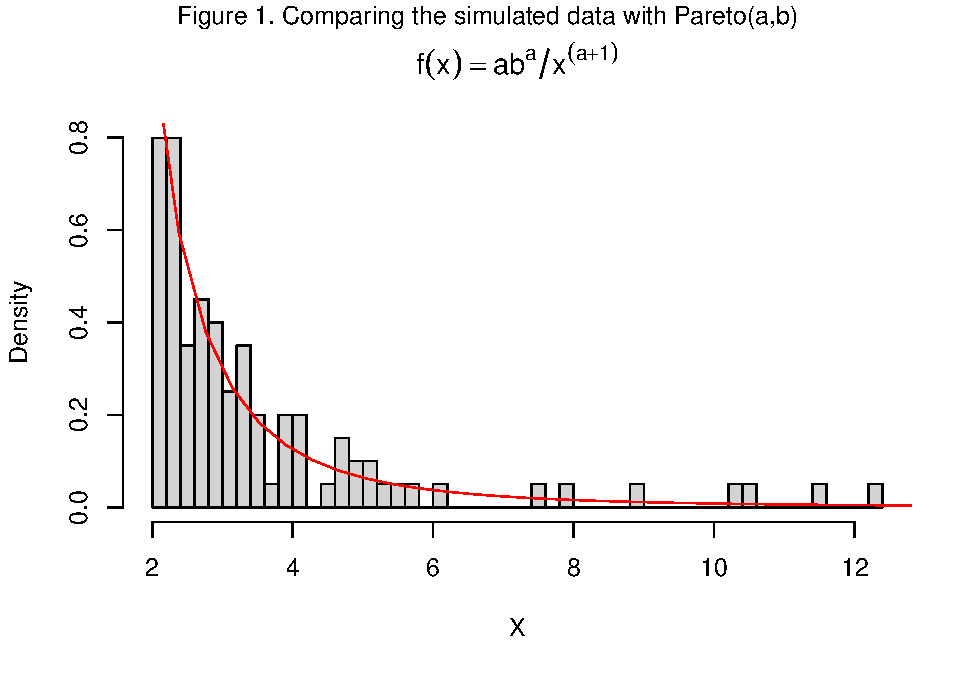
\includegraphics[width=1\linewidth,height=0.4\textheight]{HW_02_Chenguang_Pan_files/figure-latex/unnamed-chunk-2-1}

\hypertarget{question-02-scr-3.9}{%
\subsection{Question 02 SCR 3.9}\label{question-02-scr-3.9}}

\textbf{MY SOLUTION:}\\
This question has already given the clues to generate random variable
for the rescaled Epanechnikov kernel

\begin{Shaded}
\begin{Highlighting}[]
\SpecialCharTok{\textgreater{}} \CommentTok{\# write a function based on text\textquotesingle{}s information}
\ErrorTok{\textgreater{}}\NormalTok{ gen\_var }\OtherTok{\textless{}{-}} \ControlFlowTok{function}\NormalTok{(n)\{ }\CommentTok{\# n is the sample size}
\SpecialCharTok{+}\NormalTok{   U\_1 }\OtherTok{\textless{}{-}} \FunctionTok{runif}\NormalTok{(n, }\SpecialCharTok{{-}}\DecValTok{1}\NormalTok{, }\DecValTok{1}\NormalTok{)}
\SpecialCharTok{+}\NormalTok{   U\_2 }\OtherTok{\textless{}{-}} \FunctionTok{runif}\NormalTok{(n, }\SpecialCharTok{{-}}\DecValTok{1}\NormalTok{, }\DecValTok{1}\NormalTok{)}
\SpecialCharTok{+}\NormalTok{   U\_3 }\OtherTok{\textless{}{-}} \FunctionTok{runif}\NormalTok{(n, }\SpecialCharTok{{-}}\DecValTok{1}\NormalTok{, }\DecValTok{1}\NormalTok{)}
\SpecialCharTok{+}\NormalTok{   U\_output }\OtherTok{\textless{}{-}} \FunctionTok{c}\NormalTok{()}
\SpecialCharTok{+}   \ControlFlowTok{for}\NormalTok{ (i }\ControlFlowTok{in} \FunctionTok{c}\NormalTok{(}\DecValTok{1}\SpecialCharTok{:}\NormalTok{n)) \{}
\SpecialCharTok{+}     \ControlFlowTok{if}\NormalTok{ (}\FunctionTok{abs}\NormalTok{(U\_3[i]) }\SpecialCharTok{\textgreater{}} \FunctionTok{abs}\NormalTok{(U\_2[i]) }\SpecialCharTok{\&} 
\SpecialCharTok{+}         \FunctionTok{abs}\NormalTok{(U\_3[i]) }\SpecialCharTok{\textgreater{}} \FunctionTok{abs}\NormalTok{(U\_1[i]))}
\SpecialCharTok{+}\NormalTok{       \{U\_output[i] }\OtherTok{\textless{}{-}}\NormalTok{ U\_2[i]\} }
\SpecialCharTok{+}     \ControlFlowTok{else} 
\SpecialCharTok{+}\NormalTok{       \{U\_output[i] }\OtherTok{\textless{}{-}}\NormalTok{ U\_3[i]\}}
\SpecialCharTok{+}\NormalTok{   \}}
\SpecialCharTok{+}   \FunctionTok{return}\NormalTok{(U\_output)}
\SpecialCharTok{+}\NormalTok{ \}}
\SpecialCharTok{\textgreater{}} 
\ErrorTok{\textgreater{}} \CommentTok{\# generate 1000 data}
\ErrorTok{\textgreater{}}\NormalTok{ U\_output }\OtherTok{\textless{}{-}} \FunctionTok{gen\_var}\NormalTok{(}\DecValTok{1000}\NormalTok{)}
\SpecialCharTok{\textgreater{}} \FunctionTok{hist}\NormalTok{(U\_output, }\AttributeTok{prob =}\NormalTok{ T, }
\SpecialCharTok{+}      \AttributeTok{breaks =} \DecValTok{100}\NormalTok{, }
\SpecialCharTok{+}      \AttributeTok{xlab =} \StringTok{"x"}\NormalTok{,}
\SpecialCharTok{+}      \AttributeTok{main =} \FunctionTok{expression}\NormalTok{(}\FunctionTok{f}\NormalTok{(x)}\SpecialCharTok{==}\NormalTok{(}\DecValTok{3}\SpecialCharTok{/}\DecValTok{4}\NormalTok{)}\SpecialCharTok{*}\NormalTok{(}\DecValTok{1}\SpecialCharTok{{-}}\NormalTok{x}\SpecialCharTok{\^{}}\DecValTok{2}\NormalTok{)))}
\SpecialCharTok{\textgreater{}}\NormalTok{ x\_vec }\OtherTok{\textless{}{-}} \FunctionTok{seq}\NormalTok{(}\SpecialCharTok{{-}}\DecValTok{1}\NormalTok{,}\DecValTok{1}\NormalTok{,}\FloatTok{0.001}\NormalTok{)}
\SpecialCharTok{\textgreater{}}\NormalTok{ f\_x }\OtherTok{\textless{}{-}} \FloatTok{0.75}\SpecialCharTok{*}\NormalTok{(}\DecValTok{1}\SpecialCharTok{{-}}\NormalTok{x\_vec}\SpecialCharTok{\^{}}\DecValTok{2}\NormalTok{)}
\SpecialCharTok{\textgreater{}} \FunctionTok{lines}\NormalTok{(x\_vec, f\_x, }\AttributeTok{col=}\StringTok{"red"}\NormalTok{)}
\SpecialCharTok{\textgreater{}} \FunctionTok{mtext}\NormalTok{(}\StringTok{"Figure 2. Rescaled Epanechnikov kernel Distribution"}\NormalTok{,}
\SpecialCharTok{+}       \AttributeTok{side =} \DecValTok{3}\NormalTok{,}
\SpecialCharTok{+}       \AttributeTok{line =} \SpecialCharTok{{-}}\DecValTok{1}\NormalTok{,}
\SpecialCharTok{+}       \AttributeTok{outer =}\NormalTok{ T)}
\end{Highlighting}
\end{Shaded}

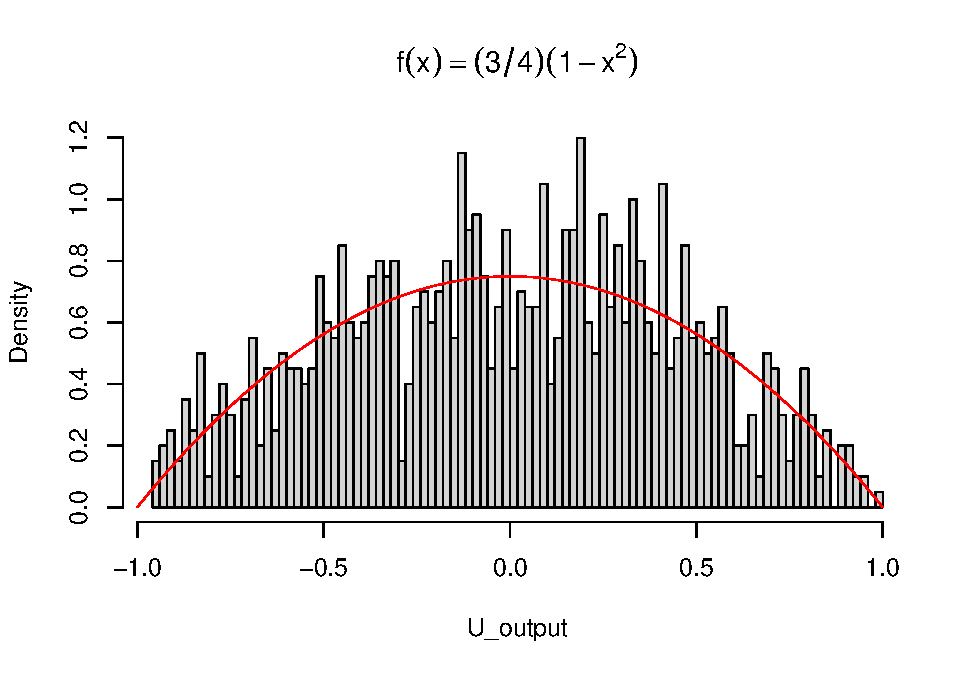
\includegraphics[width=1\linewidth,height=0.4\textheight]{HW_02_Chenguang_Pan_files/figure-latex/unnamed-chunk-3-1}

\hypertarget{question-03-scr-3.11}{%
\subsection{Question 03 SCR 3.11}\label{question-03-scr-3.11}}

\textbf{MY SOLUTION:}\\
How to better understand the mixing weights (i.e., the mixing
probabilities)? The mixing weights is about \textbf{how much} each
individual distribution contributes to the mixture
distribution(\href{https://www.statisticshowto.com/mixture-distribution/}{Stephanie
Glen. StatisticsHowTo.com}). Therefore, when constructing the mixture
function, one should not directly use the probability of each parent
distribution as a coefficient!!

\begin{Shaded}
\begin{Highlighting}[]
\SpecialCharTok{\textgreater{}} \FunctionTok{set.seed}\NormalTok{(}\DecValTok{1000}\NormalTok{)}
\SpecialCharTok{\textgreater{}}\NormalTok{ n }\OtherTok{\textless{}{-}} \DecValTok{1000}
\SpecialCharTok{\textgreater{}} \CommentTok{\# generate two vectors from normal distribution}
\ErrorTok{\textgreater{}}\NormalTok{ x1 }\OtherTok{\textless{}{-}} \FunctionTok{rnorm}\NormalTok{(n,}\DecValTok{0}\NormalTok{,}\DecValTok{1}\NormalTok{)}
\SpecialCharTok{\textgreater{}}\NormalTok{ x2 }\OtherTok{\textless{}{-}} \FunctionTok{rnorm}\NormalTok{(n,}\DecValTok{3}\NormalTok{,}\DecValTok{1}\NormalTok{)}
\SpecialCharTok{\textgreater{}} 
\ErrorTok{\textgreater{}} \CommentTok{\# use a for{-}loop to draw graphs at different mixing weights}
\ErrorTok{\textgreater{}} \FunctionTok{par}\NormalTok{(}\AttributeTok{mfrow=}\FunctionTok{c}\NormalTok{(}\DecValTok{3}\NormalTok{,}\DecValTok{2}\NormalTok{))}
\SpecialCharTok{\textgreater{}} \ControlFlowTok{for}\NormalTok{ (p1 }\ControlFlowTok{in} \FunctionTok{c}\NormalTok{(}\FloatTok{0.75}\NormalTok{, }\FloatTok{0.90}\NormalTok{, }\FloatTok{0.60}\NormalTok{, }\FloatTok{0.5}\NormalTok{, }\FloatTok{0.30}\NormalTok{, }\FloatTok{0.15}\NormalTok{))\{}
\SpecialCharTok{+}   \CommentTok{\# define the mixing prob}
\SpecialCharTok{+}\NormalTok{   p2 }\OtherTok{\textless{}{-}} \DecValTok{1} \SpecialCharTok{{-}}\NormalTok{ p1}
\SpecialCharTok{+}   \CommentTok{\# use n data from uniform distribution to construct}
\SpecialCharTok{+}   \CommentTok{\# the proportion of each parent distribution.}
\SpecialCharTok{+}\NormalTok{   u }\OtherTok{\textless{}{-}} \FunctionTok{runif}\NormalTok{(n)}
\SpecialCharTok{+}\NormalTok{   k }\OtherTok{\textless{}{-}} \FunctionTok{as.integer}\NormalTok{(u }\SpecialCharTok{\textgreater{}}\NormalTok{ p2)}
\SpecialCharTok{+}\NormalTok{   x }\OtherTok{\textless{}{-}}\NormalTok{ k }\SpecialCharTok{*}\NormalTok{ x1 }\SpecialCharTok{+}\NormalTok{ (}\DecValTok{1}\SpecialCharTok{{-}}\NormalTok{k) }\SpecialCharTok{*}\NormalTok{ x2}
\SpecialCharTok{+}   \FunctionTok{hist}\NormalTok{(x, }\AttributeTok{prob =}\NormalTok{ T, }
\SpecialCharTok{+}        \AttributeTok{breaks =} \DecValTok{50}\NormalTok{, }
\SpecialCharTok{+}        \AttributeTok{xlab =} \StringTok{"mixture x"}\NormalTok{,}
\SpecialCharTok{+}        \AttributeTok{main =} \FunctionTok{sprintf}\NormalTok{(}\StringTok{"p1=\%s, p2=\%s"}\NormalTok{, p1, p2))}
\SpecialCharTok{+}   \FunctionTok{lines}\NormalTok{(}\FunctionTok{density}\NormalTok{(x), }\AttributeTok{col=} \StringTok{"red"}\NormalTok{)}
\SpecialCharTok{+}\NormalTok{ \}}
\SpecialCharTok{\textgreater{}} \FunctionTok{mtext}\NormalTok{(}\StringTok{"Figure 3. Mixture Distributions With Different Mixing Weights"}\NormalTok{,}
\SpecialCharTok{+}       \AttributeTok{side =} \DecValTok{3}\NormalTok{,}
\SpecialCharTok{+}       \AttributeTok{line =} \SpecialCharTok{{-}}\DecValTok{1}\NormalTok{,}
\SpecialCharTok{+}       \AttributeTok{outer =}\NormalTok{ T)}
\end{Highlighting}
\end{Shaded}

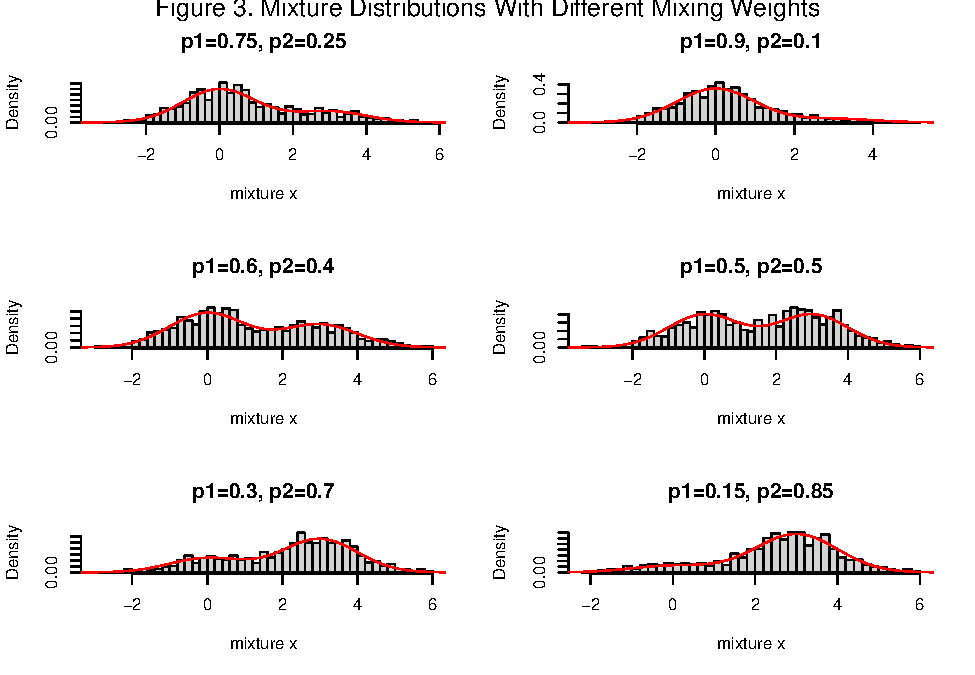
\includegraphics{HW_02_Chenguang_Pan_files/figure-latex/unnamed-chunk-4-1.pdf}
From the graphs, one can find that when the mixing weights are .5 and
.5, the mixture distribution is apparently a bimodal distribution. At
this circumstance the two samples contribute equally to the final
mixture. But this bimodal distribution might not be symmetrical because
the two parent distribution's shapes are different in variance. With
increasing in P1, the bimodal distribution will be more positively
skewed.

\end{document}
